\documentclass[12pt,french,oneside]{report}
%%%%%%%%%%%%%%%%%%%%%%%%%%%%%%%%%%%%%%%%%%%%%%%%%%%%%%
\input{preambule_2021}
%%%%%%%%%%%%%%%%%%%%%%%%%%%%%%%%%%%%%%%%%%%%%%%%%%%%%%
\portrait
%\paysage
%%%%%%%%%%%%%%%%%%%%%%%%%%%%%%%%%%%%%%%%%%%%%%%%%%%%%%

%À modifier !!!!!!!!!!!!!!!!!!!!!!!!!!!!!!!!
\newcommand{\classe}{\tmaths}
\newcommand{\anneescol}{Année 2021-2022}
\newcommand{\nomchapitre}{Vecteurs, droites et plans de l'espace}

%entête classique

\fancypagestyle{plain}{%
\fancyhf{} % vide l'en-tête et le pied~de~page.
%\fancyhead[C]{\small\textbf{\tesspe} \hfill \small \textbf{Année 2014-2015}}
\renewcommand{\headrulewidth}{0cm}
\renewcommand \headrulewidth{0pt}%
\pieddepage{\classe}{\thepage / \pageref{LastPage}}{\nomchapitre}
}

\newcommand{\tete}{
\thispagestyle{plain}
\setcounter{chapter}{5}%le chapitre en cours est alors le chapitre 3 avec \setcounter{chapter}{2}
\chapter{\nomchapitre}
\noindent 
%\vspace{-12pt}
}

\usepackage{minitoc}
\dominitoc
%%%%%%%%%%%%%%%%%%%%%%%%%%%%%%%%%%%%%%%%%%%%%%%%%%%%
%%%%%%%%%%%%%%%%%%%%%%%%%%%%%%%%%%%%%%%%%%%%%%%%%%%%
%\tikzset{domaine/.style 2 args={domain=#1:#2}}


%Options de tcolorbox pour les encadrés
\tcbuselibrary{many}
\tcbset{drop fuzzy shadow,
    enhanced,
    attach boxed title to top left={
        xshift=0.25cm,
        yshift= -2.5mm,
    },
    top=4mm,
    beforeafter skip=\baselineskip,
}

\NewEnviron{Encadre}[4][]{
\begin{tcolorbox}[colback=#1,colframe=#2,colbacktitle=#3,title=\textbf{#4}]
\raggedright
\BODY
\end{tcolorbox}
}

\newcounter{propriete}
\NewEnviron{Propriete}[3][]{
\refstepcounter{propriete}
\begin{tcolorbox}[colback=#2,colframe=gray!50,colbacktitle=blue!50,title=\textbf{Propriété#1~\thepropriete~:~#3}]
\raggedright
\BODY
\end{tcolorbox}
}

%%%%%%%%%%%%%%%%%%%%%%%%%%%%%%%%%%%%%%%%%%%%%%%%%%%%
%%%%%%%%%%%%%%%%%%%%%%%%%%%%%%%%%%%%%%%%%%%%%%%%%%%%

%%%%%%%%%%%%%%%%%%%%%%%
%% DEBUT DU DOCUMENT %%
%%%%%%%%%%%%%%%%%%%%%%%

\begin{document}
%\selectlanguage{english}
\selectlanguage{french}
\setlength\parindent{0mm}
\tete 		%entête classique

\renewcommand \footrulewidth{0.2pt}%
\renewcommand \headrulewidth{0pt}%
\pagestyle{fancy}
\fancyhf{}
\pieddepage{\classe}{\thepage / \pageref{LastPage}}{\nomchapitre}

%%%%%%%%%%%%%%%%%%%%%%%%%%%%%%%%%%%%%%%%%%%%%%%%%%%%%%%%%%%%
\begin{spacing}{1.2}
%%%%%%%%%%%%%%%%%%%%%%%%%%%%%%%%%%%%%%%%%%%%%%%%%%%%%%%%%%%%
%\pagecolor{gray!80}\color{white}%on voit mal le sommaire sur fond noir
%%%%%%%%%%%%%%%%%%%%%%%%%%%%%%%%%%%%%%%%%%%%%%%%%%%%
\setcounter{minitocdepth}{3}    % Show until subsubsections in minitoc
\minitoc\faketableofcontents
%%%%%%%%%%%%%%%%%%%%%%%%%%%%%%%%%%%%%%%%%%%%%%%%%%%%%%%%%%%%%%%%
\section*{Pré-requis}
%%%%%%%%%%%%%%%%%%%%%%%%%%%%%%%%%%%%%%%%%%%%%%%%%%%%%%%%%%%%%%%%

Les packages \verb~environ~ et \verb~tcolorbox~.

Le code suivant dans le préambule :

\begin{verbatim}
\tcbuselibrary{many}
\tcbset{drop fuzzy shadow,
    enhanced,
    attach boxed title to top left={
        xshift=0.25cm,
        yshift= -2.5mm,
    },
    top=4mm,
    beforeafter skip=\baselineskip,
}

\NewEnviron{Encadre}[4][]{
\begin{tcolorbox}[colback=#1,colframe=#2,colbacktitle=#3,title=\textbf{#4}]
\raggedright
\BODY
\end{tcolorbox}
}
\end{verbatim}


%%%%%%%%%%%%%%%%%%%%%%%%%%%%%%%%%%%%%%%%%%%%%%%%%%%%
\section*{Exemples}
%%%%%%%%%%%%%%%%%%%%%%%%%%%%%%%%%%%%%%%%%%%%%%%%%%%%


\begin{Encadre}[white]{gray!50}{blue!50}{Titre}
Essai avec le package tcolorbox.

Tu peux changer la couleur du fond du titre, de l'encadré, de l'intérieur de l'encadré facilement.
\end{Encadre}

\textbf{Anciens encadrés}

\begin{Cadre}
Ancien encadré blanc
\end{Cadre}

\begin{CadreColor}
Ancien encadré couleur
\end{CadreColor}





\textbf{Nouveaux environnements}


\begin{Propriete}[]{red!10}{Titre}
Essai avec le package tcolorbox.

Tu peux changer la couleur du fond du titre, de l'encadré, de l'intérieur de l'encadré facilement.
\end{Propriete}

\begin{Propriete}[s]{red!10}{Titre}
Essai avec le package tcolorbox.

\begin{center}
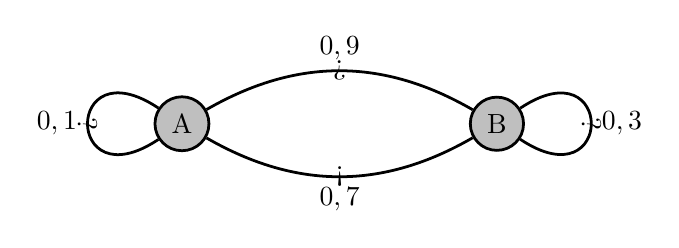
\begin{tikzpicture}[scale=1]
\tikzstyle{every path}=[line width=1pt];
\node [draw,circle,fill=gray!50] (A) at (0,0) {A};
\node [draw,circle,fill=gray!50] (B) at (4,0) {B};
\draw (A) to [bend left]  node[midway,sloped,above] {$0,9$} node[midway,sloped]{>} (B);
\draw (B) to [bend left] node[midway,sloped,below] {$0,7$} node [midway,sloped] {<} (A);
\draw (B) .. controls +(1.5,-1) and +(1.5,1) .. node[midway,right]{$0,3$} node [midway,sloped] {>} (B) ;
\draw (A) .. controls +(-1.5,-1) and +(-1.5,1) .. node[midway,left]{$0,1$} node [midway,sloped] {>} (A) ;
\end{tikzpicture}
\end{center}

Tu peux changer la couleur du fond du titre, de l'encadré, de l'intérieur de l'encadré facilement.

\begin{center}

\begin{tikzpicture}
\tkzTabInit[color,lgt=2.5,espcl=6,colorC=blue!20,colorV=blue!20]
{$x$/1,$f'(x)$/1,Variations\\de $f$/1.5}
{$0$,{$1,5$},$+\infty$}
\tkzTabLine{,-,z,+,}
\tkzTabVar{+/,-/$0$,+/}
\end{tikzpicture}
\end{center}

Aucun souci pour insérer des figure TikZ !!!
\end{Propriete}



%%%%%%%%%%%%%%%%%%%%%%%%%%%%%%%%%%%%%%%%%%%%%%%%%%%%%%%%%%%%
\end{spacing}
%%%%%%%%%%%%%%%%%%%%%%%%%%%%%%%%%%%%%%%%%%%%%%%%%%%%%%%%%%%%
%%%%%%%%%%%%%%%%%%%%%
%% FIN DU DOCUMENT %%
%%%%%%%%%%%%%%%%%%%%%
\end{document}